\documentclass[tikz,border=4pt]{standalone}
\usetikzlibrary{arrows.meta,positioning,fit}
\begin{document}
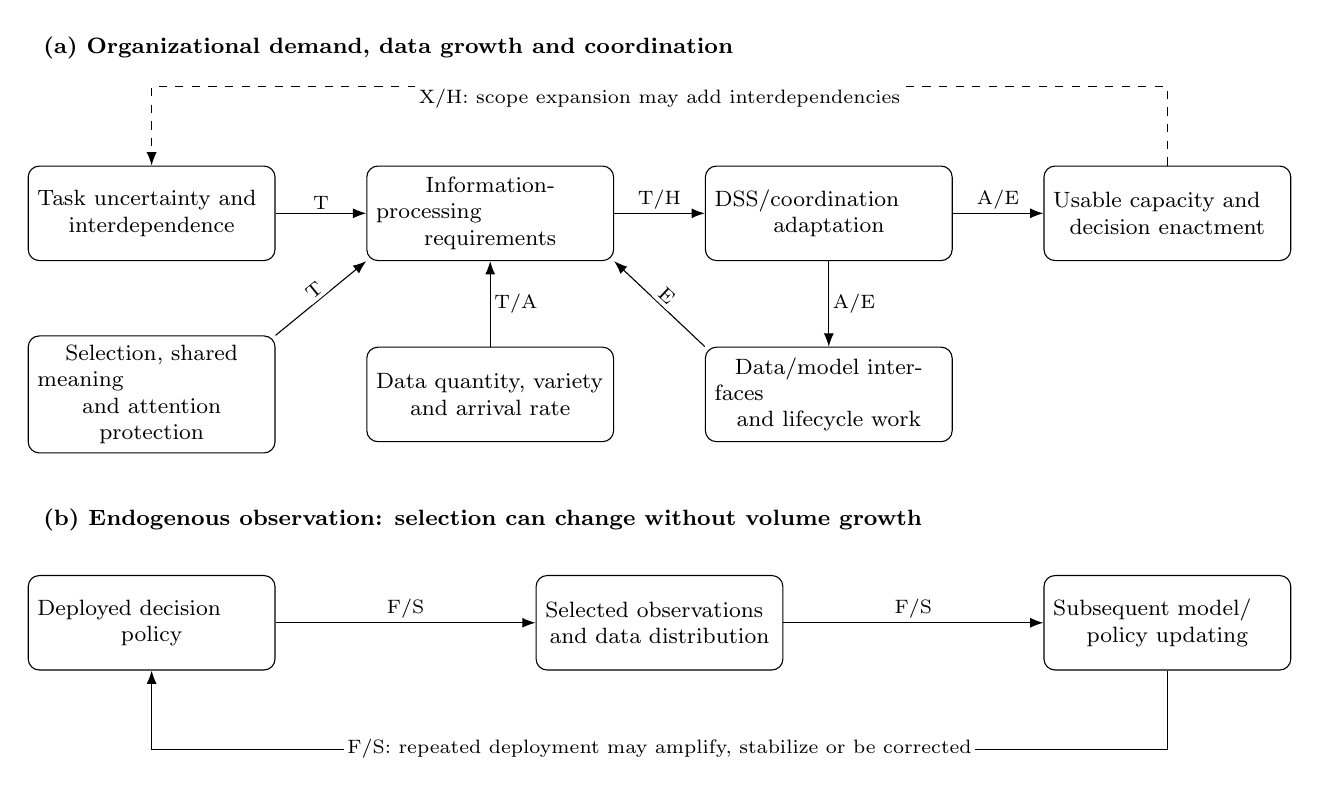
\begin{tikzpicture}[>=Latex, every node/.style={font=\footnotesize}, box/.style={draw,rounded corners,align=center,text width=29mm,minimum height=12mm}, lab/.style={font=\scriptsize,align=center,fill=white,inner sep=1.3pt}]
\node[font=\bfseries\footnotesize,anchor=west] at (-1.5,2.1) {(a) Organizational demand, data growth and coordination};
\node[box] (c) at (0,0) {Task uncertainty and\newline interdependence};
\node[box] (r) at (4.3,0) {Information-processing\newline requirements};
\node[box] (a) at (8.6,0) {DSS/coordination\newline adaptation};
\node[box] (w) at (12.9,0) {Usable capacity and\newline decision enactment};
\node[box] (b) at (0,-2.3) {Selection, shared meaning\newline and attention protection};
\node[box] (v) at (4.3,-2.3) {Data quantity, variety\newline and arrival rate};
\node[box] (g) at (8.6,-2.3) {Data/model interfaces\newline and lifecycle work};
\draw[->] (c) -- node[lab,above] {T} (r);
\draw[->] (r) -- node[lab,above] {T/H} (a);
\draw[->] (a) -- node[lab,above] {A/E} (w);
\draw[->] (a) -- node[lab,right] {A/E} (g);
\draw[->] (g.north west) -- node[lab,sloped,above] {E} (r.south east);
\draw[->] (v) -- node[lab,right] {T/A} (r);
\draw[->] (b.north east) -- node[lab,sloped,above] {T} (r.south west);
\draw[->,dashed] (w.north) -- ++(0,10mm) -| (c.north);
\node[lab] at (6.45,1.45) {X/H: scope expansion may add interdependencies};
\node[font=\bfseries\footnotesize,anchor=west] at (-1.5,-3.9) {(b) Endogenous observation: selection can change without volume growth};
\node[box] (p) at (0,-5.2) {Deployed decision\newline policy};
\node[box] (d) at (6.45,-5.2) {Selected observations\newline and data distribution};
\node[box] (u) at (12.9,-5.2) {Subsequent model/\newline policy updating};
\draw[->] (p) -- node[lab,above] {F/S} (d);
\draw[->] (d) -- node[lab,above] {F/S} (u);
\draw[->] (u.south) -- ++(0,-10mm) -| (p.south);
\node[lab] at (6.45,-6.8) {F/S: repeated deployment may amplify, stabilize or be corrected};
\end{tikzpicture}
\end{document}
